\chapter{Sensors \& Data Collection}\label{chapter:data-collection}
This chapter describes the measurement and collection of readings to determine the orientation of the accelerometer, gyroscope, and magnetometer.
After determining the orientation of the accelerometer, additional data of the user movement is recorded.
Hereafter, the gyroscope and the magnetometer are described, and readings from these sensors are used to determine the angle of the device.
The data will be examined to determine how the movement of the user affects the acceleration.

\section{Accelerometer}\label{section:accelerometer}
Before starting the implementation of the application, the accelerometer of the phone should be examined. 
Knowing the orientation of the accelerometer axis in the phone is important in the implementation of dead reckoning.
As mentioned in \secref{section:limitations}, the phone will be in held in a fixed position when the game is played. 
Which means that sideways movements will be tracked along one axis, and will be used to move the paddle accordingly.
To find the axis orientation, tests have been made by moving the phone in specific directions and looking at the data output. 
The orientation of the accelerometer axis' can be seen in \figref{figure:axis-orientation}.

\begin{figure}[h]
	\centering
	\includegraphics[scale=0.5]{media/phone-rotation/phone-axistocality}
	\caption{The orientation of the accelerometer.}
	\label{figure:axis-orientation}
\end{figure}

Another functionality that needs testing is how the data behaves when the phone is rotated manually around the different axis', which is needed because when the user holds the phone it will be tilted.
In \figref{figure:phone-rotate-y-axis-graph}, a graph shows the accelerations of the axis when the phone is rotated counter-clockwise around the y-axis from the position shown in \figref{figure:axis-orientation}, other recordings was performed for rotation around the other axis' but has been omitted as it does not give new insight to the understanding of the accelerometer.
%pull 90 grader
\begin{figure}[h]
\centering
	\includegraphics[scale=0.45, trim=0cm 2cm 0cm 2cm]{media/gnuplot/rotation.pdf}
	\caption{Acceleration graph recorded for rotating $90^\circ$ around the y-axis. (Blue = x, Black = y, Green = z)}
	\label{figure:phone-rotate-y-axis-graph}
\end{figure}
When the user is holding the phone as in \figref{figure:axis-orientation}, the accelerations, in the device's y-axis, of a step to the left and to the right can be seen in \figref{figure:step-left-and-right}.
The acceleration is measured in gravitational force (g-force) and the time in milliseconds, where $1 g$ is the gravitational pull.
The accelerometer for the chosen phone have a measurement limit between $-2 g$ and $2 g$.

\begin{figure}[H]
	\centering	
	\includegraphics[scale=0.45, trim=0cm 2cm 0cm 2cm]{media/gnuplot/tokew.pdf}
	\caption{A graph showing a left, blue, and a right, red, step.}
	\label{figure:step-left-and-right}
\end{figure}

%Dette billede kan også ses udfra det første billede!
%\begin{figure}
%	\centering
%	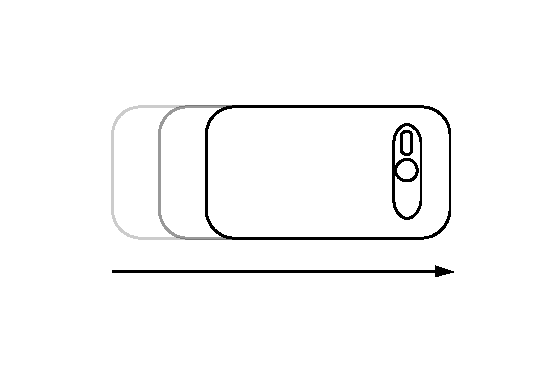
\includegraphics{media/phone-rotation/phone-horizontality}
%	\caption{Phone moving along the y-axis. (Back of the phone)}
%	\label{key}
%\end{figure}



\section{Gyroscope}\label{section:gyroscope}
%hvad er det?
%hvordan virker det. vis tegning.
%hvad kan det bruges til?
%hvad er drifting. hvorfor drifter den? hvordan fixer man det? PIETER JAN!

The gyroscope measures the rotational velocity ($rad/s$), meaning how much the orientation of the phone has changed since last reading.
The orientations of the phone is referred to as \textit{Pitch}, \textit{Roll}, and \textit{Yaw} and is measured around the axes x, y, and z, respectively as illustrated in \figref{figure:phone-gyroscope}. 
As an example, if the user rotates the device $20^\circ$ around its x-axis, Pitch will, over the course of the action, accumulate to $0.35$ radians, whereas Roll and Yaw remain unaffected.

\begin{figure}[h]
	\centering
	\includegraphics[scale=0.5]{media/phone-rotation/phone-gyroscope}
	\caption{Pitch, Roll and Yaw illustrated.}
	\label{figure:phone-gyroscope}
\end{figure}

The gyroscope can be used in the application to accommodate for tilting the phone while playing.
Without this accommodation the gravitational pull would affect the acceleration-reading of the y-axis, when the phone has a yaw-rotation.
Furthermore, if the phone has a pitch-rotation, the acceleration in the y-axis is smaller than intended, which can be corrected using the gyroscope and is further explained in \secref{section:SensorFusion}.

When using the gyroscope, the accumulation of each gyroscope reading is needed to determine the correct angle that the phone is tilted. 
Due to noise in the gyroscope readings, the accumulated value will be inaccurate.
The inaccuracy can cause drifting, which means the gyroscope cannot track when the system is back to its original position.
To avoid drifting, the gyroscope can be utilised together with the accelerometer to correct the uncertainties of the gyroscope \citep{misc:pieter-jan, misc:balance-filter}.

To test how much the angle drifts, the device was positioned on a flat, undisturbed surface for 3 minutes.
The recording can be seen in \figref{figure:phone-complementary-filter} where one graph illustrates raw data received from the gyroscope, and another graph illustrates the same dataset run through a complementary filter.

\begin{figure}[h]
	\centering
	\includegraphics[scale=0.45, trim = 0cm 2cm 0cm 2cm]{media/gnuplot/compfilter.pdf}
	\caption{The complementary-filter over a 3 minute period.}
	\label{figure:phone-complementary-filter}
\end{figure}

As is clearly evident by the graphs, implementing a complementary filter would greatly increase the accuracy of the application.
The sensor fusion is implemented using a complementary filter to have the acceleration reading adjust the accumulated angle of the gyroscope.
The formula is as follows:

\begin{equation*}
	angle = \alpha*(angle + gyro * \Delta t) + (1 - \alpha)(angle_{acc})
\end{equation*}
where,
\begin{enumerate}
	\item[]
\begin{enumerate}
	\item[$angle$] is the accumulated angle.
	\item[$\alpha$] is the coefficient which determine how much each sensor affects the result.
	\item[$gyro$] is the gyroscope reading measured in $rad/s$.
	\item[$angle_{acc}$] is the angle, determined by the acceleration, measured in $rad$ and found using atan2 function.
\end{enumerate}
\end{enumerate}

\section{Magnetometer}\label{section:magnetometer}
The smartphone moves along the y-axis, but sometimes the phone rotates around the x- and z-axis when the player moves, which gives a smaller acceleration in the y-axis. 
To correct the accelerometer reading, the magnetometer can be used.
Using the magnetometer, the initial orientation can be found, which then can be compared to the current orientation to find the angle difference.
To find the orientation of the magnetometer, the phone was held in four different positions. 

Drawings of these positions can be seen in \figref{figure:magnetometer-headings}.
Each drawing and its corresponding caption, shows the geographical north pole and the heading of the smartphone.
\figref{figure:position-yz} illustrates how the phone should be held when the application is in use and the +z-axis is directed north. 
The magnetometer showed an angle of $270^\circ$, which is west, hereby, it could be concluded that the orientation of the magnetometer followed the -y-axis.
When the phone is tilted as seen in \figref{figure:position-xz} and \figref{figure:position-xy}, the y-axis was now in a vertical direction and the +z-axis was directed north, the magnetometer gave an angle of $0^\circ$ and $90\circ$, respectively. 
This angle indicated that when the y-axis is at a vertical direction the +z-axis becomes the direction in which the magnetometer measures its angle.\fxwarning{Det kan man ikk konkluderer udfra billederne, der mangler et forsøg hvor y peger nedad og z er vendt væk fra nord.}
\figref{figure:position-yx} were used to confirm that whenever the y-axis is in a horizontal direction, the -y-axis is the direction in which the magnetometer measures its angle.
When the different directions of the magnetometer are known, they can be used to correct the affected readings from the acceleration in the y-axis.

%Direction Hvilken vej noget vender/peger
%Heading er et resultat
%Orientaion hvordan telefonen er bygget/orienteret
%Allignment hvordan man står i forhold til noget

\begin{figure}[H]
	\centering
	%---- linebreak	
	\begin{subfigure}[b]{0.45\textwidth}
		\centering
		\includegraphics[scale = 0.4]{media/phone-rotation/phone-compass-a}
        \caption[caption]{The side of the phone.\\Magnetometer reading: $270^{\circ}$.}
		\label{figure:position-yz}
	\end{subfigure}
	\qquad
	\begin{subfigure}[b]{0.45\textwidth}
		\centering
		\includegraphics[scale = 0.4]{media/phone-rotation/phone-compass-b}
        \caption[caption]{The top of the phone.\\Magnetometer reading: $0^{\circ}$.}
		\label{figure:position-xz}
	\end{subfigure}
	%---- linebreak
	\begin{subfigure}[b]{0.45\textwidth}
		\centering
		\includegraphics[scale = 0.4]{media/phone-rotation/phone-compass-c}
        \caption[caption]{The front of the phone, in landscape mode.\\Magnetometer reading: $270^{\circ}$.}
		\label{figure:position-yx}
	\end{subfigure}
	\qquad
	\begin{subfigure}[b]{0.45\textwidth}
		\centering
		\includegraphics[scale = 0.4]{media/phone-rotation/phone-compass-e}
        \caption[caption]{The top of the phone.\\Magnetometer reading: $90^{\circ}$.}

		\label{figure:position-xy}
	\end{subfigure}		
	\caption{The orientation of the phone and its corresponding magnetometer reading. All drawings are seen from above.}
	\label{figure:magnetometer-headings}
\end{figure}

\section{Data logger}\label{section:datalogger}
All the data in this project has been logged, using a Nokia Lumia 820 running Windows Phone 8.
The data logger has been used to understand the output of the phone's different sensors.
It works by recording output from the accelerometer, the gyroscope, and the magnetometer, the collected data can then be sent to a web-service, which stores the data in a database.
To make sure that the data logger does not overburden the database with update-requests, all the sensor-data is stored locally, and sent to the web-service once recording is complete.
%The data is sent by a web client, and it is therefore possible to sent multiple data sets together.
The data has been sent through a web-service because Windows Phone 8 does not offer a framework which works directly with MySQL.
